\documentclass[a4paper,oneside,brazil,11pt,a4paper,openright,titlepage,usenames,dvipsnames]{book}
% Classe alternativa, apropriada para impressão frente-verso. Inclui páginas em branco de forma que capítulos sempre tenham início na página à direita:
% \documentclass[11pt,a4paper,openright,titlepage]{book}

\usepackage[utf8]{inputenc}
\usepackage[T1]{fontenc}
\usepackage[brazilian]{babel}
\usepackage{lmodern}
\usepackage{array}
\usepackage{verbatim}
\usepackage{calc}
\usepackage{textcomp}
\usepackage{gensymb}
\usepackage{amsfonts}
\usepackage{amsmath}
\usepackage[thmmarks,amsmath]{ntheorem}%\usepackage{amsthm}
\usepackage{amssymb}
\usepackage{graphicx}
\usepackage{float}
\usepackage[]{subfigure}
\usepackage{epsfig}
\usepackage{boxedminipage}
\usepackage{geometry}
\usepackage{theorem}
\usepackage{fancybox}
\usepackage{fancyhdr}
\usepackage{ifthen}
\usepackage{url}
\usepackage{afterpage}
\usepackage{color}
\usepackage{colortbl}
\usepackage{rotating}
\usepackage{makeidx}
\usepackage{indentfirst}
\usepackage{import}
\usepackage{enumitem}

% Escolher um dos seguintes formatos: (ft1unb) ou (ft2unb)
\usepackage{ft2unb} % ft2unb segue padrão de fontes do LaTeX;

\makeindex

\makeatother

\begin{document}
\setcounter{secnumdepth}{3}
\setcounter{tocdepth}{2}
\pagestyle{empty}

\grau{Engenheiro de Controle e Automação}

\tipodemonografia{TRABALHO DE GRADUAÇÃO}

% Título
\titulolinhai{RISC-V SiMPLE}
\titulolinhaii{}
\titulolinhaiii{}
\titulolinhaiv{}


% Autores
\autori{Arthur de Matos Beggs}
\autorii{}
\autoriii{}


% Membros da banca
\membrodabancai{Prof.\ Marcus Vinicius Lamar, CIC/UnB}
\membrodabancaifuncao{Orientador}

\membrodabancaii{Prof.\ Ricardo Pezzuol Jacobi, CIC/UnB}
\membrodabancaiifuncao{Co-Orientador}

\membrodabancaiii{}
\membrodabancaiiifuncao{}

\membrodabancaiv{}
\membrodabancaivfuncao{}

\membrodabancav{}
\membrodabancavfuncao{}


% Data de defesa
\mes{Dezembro}
\ano{2018}


% Comandos para criar a capa e a página de assinaturas
\capaprincipal{}
\capaassinaturas{}


% Ficha Catalográfica
\noindent \textbf{FICHA CATALOGRÁFICA}

\noindent %
\fbox{\begin{minipage}[t]{1\columnwidth}%
ARTHUR, DE MATOS BEGGS

RISC-V SiMPLE,

\medskip{}


{[}Distrito Federal{]} 2018.

\medskip{}


x, 101p., 297 mm (FT/UnB, Engenheiro, Controle e Automação, 2018).
Trabalho de Graduação \textendash{} Universidade de Brasília.Faculdade
de Tecnologia.

\medskip{}


1. RISC-V\hfill{}2. ???\hfill{}

\medskip{}


I. Mecatrônica/FT/UnB\hfill{}II. Título (Série)\hfill{}

%
\end{minipage}}

\noindent \medskip{}


\noindent \textbf{REFERÊNCIA BIBLIOGRÁFICA}

BEGGS, ARTHUR DE MATOS, (2018). RISC-V SiMPLE. Trabalho de Graduação
em Engenharia de Controle e Automação, Publicação FT.TG-$n^{\circ}022$,
Faculdade de Tecnologia, Universidade de Brasília, Brasília, DF, 101p.

\noindent \bigskip{}


\noindent \textbf{CESSÃO DE DIREITOS}

\noindent AUTOR: Arthur de Matos Beggs

TÍTULO DO TRABALHO DE GRADUAÇÃO: RISC-V SiMPLE.

\noindent \medskip{}


\noindent GRAU: Engenheiro\hfill{}ANO: 2018\hfill{}

\noindent \medskip{}


É concedida à Universidade de Brasília permissão para reproduzir cópias
deste Trabalho de Graduação e para emprestar ou vender tais cópias
somente para propósitos acadêmicos e científicos. O autor reserva
outros direitos de publicação e nenhuma parte desse Trabalho de Graduação
pode ser reproduzida sem autorização por escrito do autor.

\noindent \bigskip{}


\noindent \rule[0.5ex]{1\columnwidth}{1pt}

\noindent Arthur de Matos Beggs

\noindent SHCGN 703 Bl G Nº 120, Asa Norte

\noindent 70730-707 Brasília \textendash{} DF \textendash{} Brasil.



% Dedicatória
\frontmatter

\dedicatoriaautori{Dedico ao pato de borracha especialista em TI que sempre me ajuda a depurar meus códigos.}
\dedicatoriaautorii{}
\dedicatoriaautoriii{}

\dedicatoria{}


% Agradecimentos
\agradecimentosautori{Agradecimentos!}
\agradecimentosautorii{}
\agradecimentosautoriii{}

\agradecimentos{}


\resumo{resumo}{Resumo!

\medskip{}


Palavras Chave: RISC-V

}\vspace*{2cm}


\resumo{Abstract}{Abstract!

\medskip{}


Keywords: RISC-V

}

% Listas de conteúdo, figuras e tabelas
\sumario{}
\listadefiguras{}
\listadetabelas{}


% Lista de Símbolos
%TCIDATA{LaTeXparent=0,0,these.tex}


%\chapter*{\setfontarial\mdseries LISTA DE SÍMBOLOS} % se usar ft1unb.sty, descomente esta linha



\chapter*{LISTA DE SÍMBOLOS}

% se usar ft2unb.sty, descomente esta linha



\subsection*{Símbolos Latinos}

\begin{tabular}{p{0.1\textwidth}p{0.63\textwidth}>{\PreserveBacklash\raggedleft}p{0.15\textwidth}}
$v$  & Velocidade linear  & {[}m/s{]}\tabularnewline
\end{tabular}


\subsection*{Símbolos Gregos}

\begin{tabular}{p{0.1\textwidth}p{0.63\textwidth}>{\PreserveBacklash\raggedleft}p{0.15\textwidth}}
$\omega$ & Velocidade angular & {[}rad/s{]}\tabularnewline
\end{tabular}


\subsection*{Grupos Adimensionais}

\begin{tabular}{p{0.1\textwidth}p{0.8\textwidth}}
i, k & Contador\tabularnewline
\end{tabular}


\subsection*{Subscritos}

\begin{tabular}{p{0.1\textwidth}p{0.8\textwidth}}
$ref$  & referência \tabularnewline
$fer$  & ferramenta \tabularnewline
$sis$  & sistema \tabularnewline
$des$  & desejado\tabularnewline
\end{tabular}


\subsection*{Sobrescritos}

\begin{tabular}{p{0.1\textwidth}p{0.8\textwidth}}
$\cdot$  & Variação temporal \tabularnewline
$-$  & Valor médio \tabularnewline
\end{tabular}


\subsection*{Siglas}

\begin{tabular}{p{0.1\textwidth}p{0.8\textwidth}}
PCI  & \textit{Peripheral Component Interconnect}\tabularnewline
CPU & Unidade Central de Processamento - \textit{Central Processing Unit} \tabularnewline
AO & Saída Analógica - \textit{Analog Out}\tabularnewline
DO & Saída Digital - \textit{Digital Out}\tabularnewline
CS & Seletor de \textit{Chip - Chip Select}\tabularnewline
SC & Sem Conexão\tabularnewline
P.I. & Placa de Interface\tabularnewline
ICW & \textit{Initialization Command Words}\tabularnewline
OCW & \textit{Operational Control Word}\tabularnewline
\end{tabular}



% Corpo Principal
\mainmatter{}
\setcounter{page}{1}
\pagenumbering{arabic}
\pagestyle{plain}


\chapter{Introdução}

\label{CapIntro}

% Resumo opcional. Comentar se não usar.
\resumodocapitulo{Resumo opcional}


\section{Contextualização}

Contextualizar.

Conforme \cite{article:dummy}, vide a Tabela \ref{tab:Descrever-tabela}.
Assim sendo, observe a Figura \ref{fig:Descrever-figura.}.
\begin{table}[h]
\begin{centering}
\begin{tabular}{|c|c|c|c|c|}
\hline
 &  &  &  & \tabularnewline
\hline
\hline
 &  &  &  & \tabularnewline
\hline
 &  &  &  & \tabularnewline
\hline
 &  &  &  & \tabularnewline
\hline
 &  &  &  & \tabularnewline
\hline
\end{tabular}
\par\end{centering}

\label{tab:Descrever-tabela}Descrever tabela.


\end{table}


\begin{figure}[h]
\begin{centering}

\includegraphics[width=0.4\columnwidth]{figs/capa_fundo}
\par\end{centering}

\label{fig:Descrever-figura.}Descrever figura.


\end{figure}



\section{Definição do problema}

Definir problema.


\section{Objetivos do projeto}

Objetivos.


\section{Resultados obtidos}

Resultados.


\section{Apresentação do manuscrito}

Apresentar.

\chapter{A \textit{ISA RISC-V}}\label{CapISA}

% Resumo opcional. Comentar se não usar.
%\resumodocapitulo{Resumo opcional}

    \section{Visão Geral da Arquitetura}

        {A \textit{ISA RISC-V} é uma arquitetura modular, sendo o módulo base de operações com inteiros mandatório em qualquer implementação. Os demais módulos são extensões de uso opcional. A arquitetura não suporta \textit{branch delay slots} e aceita instruções de tamanho variável. A codificação das instruções de tamanho variável é mostrada na Figura~\ref{fig:riscv_var_length}. As instruções presentes no módulo base correspondem ao mínimo necessário para emular por \textit{software} as demais extensões (com exceção das operações atômicas).}

        \begin{figure}[H]
        \centering
            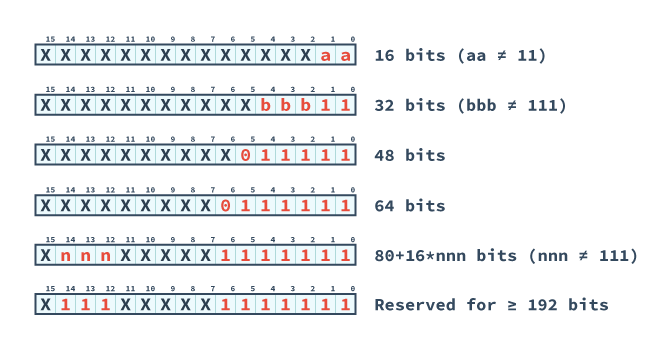
\includegraphics[width=1\linewidth]{figs/RV_InstructionLength.png}
            \caption{Codificação de instruções de tamanho variável da arquitetura \textit{RISC-V}.}\label{fig:riscv_var_length}
        \end{figure}

        \clearpage

        {A nomenclatura do conjunto de instruções implementado segue a seguinte estrutura:}

        \begin{itemize}[leftmargin=20mm]
            \item {As letras ``RV'';}
            \item {A largura dos registradores do módulo Inteiro;}
            \item {A letra ``I'' representando a base Inteira. Caso o subconjunto Embarcado (\textit{Embedded}) seja implementado, substitui-se pela letra ``E'';}
            \item {Demais letras identificadoras de módulos opcionais.}
        \end{itemize}

        {Assim, uma implementação com registradores de 64 bits somente com o módulo base de Inteiros é denominado ``RV64I''.}


        \section{Módulo Inteiro}

            {}


        \section{Extensões}

            \subsection{Extensão M}

                {}


            \subsection{Extensão A}

                {}


            \subsection{Extensão F}

                {}


            \subsection{Extensão D}

                {}


            \subsection{Outras Extensões}

                {}

    \section{Arquitetura Privilegiada}

        {}


    \section{Formatos de Instruções}

        \begin{figure}[H]
        \centering
            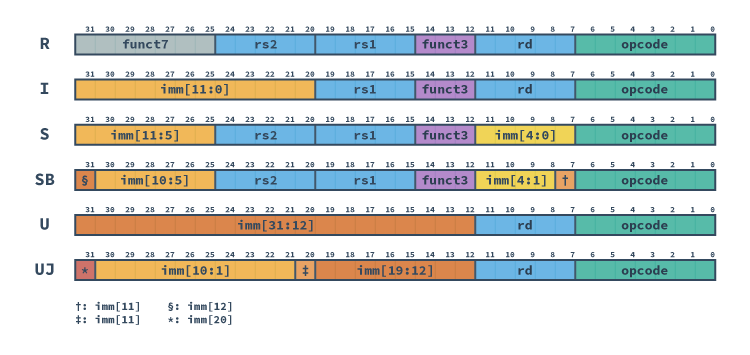
\includegraphics[width=1\linewidth]{figs/RV_Formats.png}
            \caption{Formatos de Instruções da \textit{ISA RISC-V}.}\label{fig:riscv_formats}
        \end{figure}


        % \begin{figure}[H]
        % \centering
        %     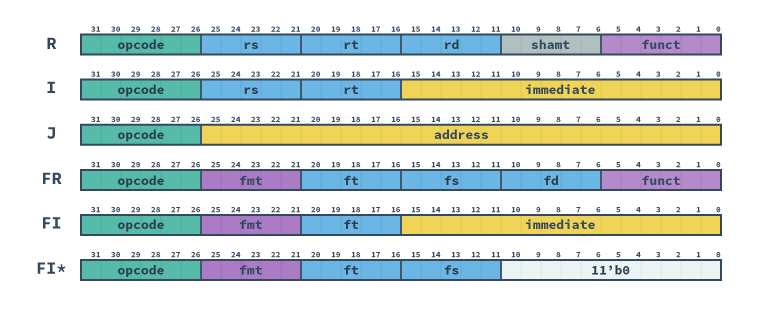
\includegraphics[width=1\linewidth]{figs/MIPS_Formats.png}
        %     \caption{Formatos de Instruções da \textit{ISA MIPS32}.}\label{fig:mips_formats}
        % \end{figure}


    \section{Formatos de Imediatos}

        \begin{figure}[H]
        \centering
            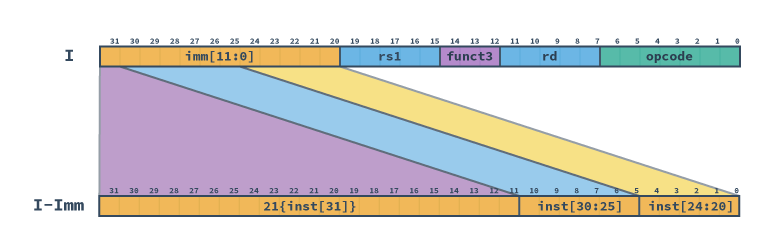
\includegraphics[width=1\linewidth]{figs/RV_I_Imm.png}
            \caption{Formação do Imediato de tipo I.}\label{fig:riscv_i_imm}
        \end{figure}

        \begin{figure}[H]
        \centering
            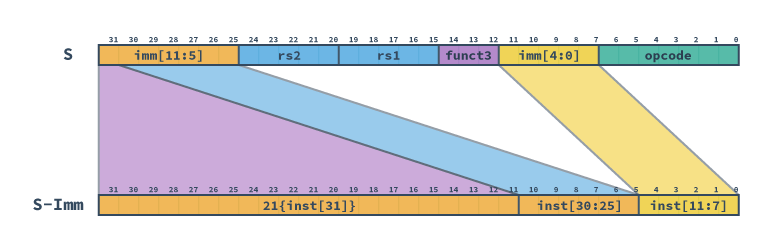
\includegraphics[width=1\linewidth]{figs/RV_S_Imm.png}
            \caption{Formação do Imediato de tipo S.}\label{fig:riscv_s_imm}
        \end{figure}

        \begin{figure}[H]
        \centering
            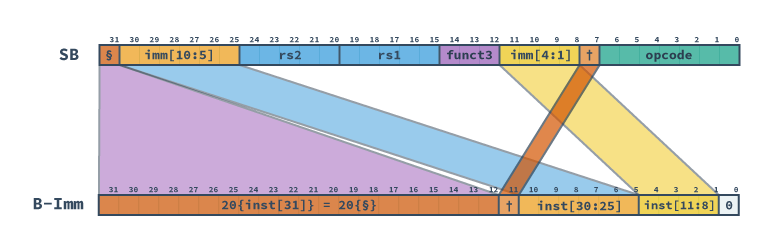
\includegraphics[width=1\linewidth]{figs/RV_B_Imm.png}
            \caption{Formação do Imediato de tipo B.}\label{fig:riscv_b_imm}
        \end{figure}

        \begin{figure}[H]
        \centering
            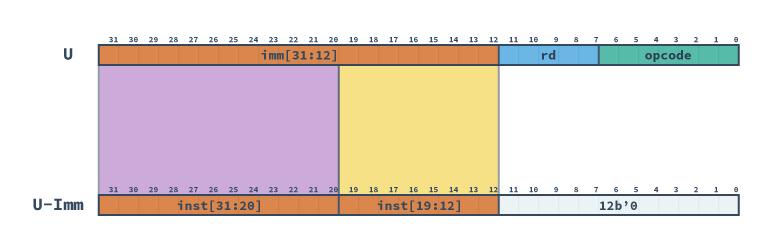
\includegraphics[width=1\linewidth]{figs/RV_U_Imm.png}
            \caption{Formação do Imediato de tipo U.}\label{fig:riscv_u_imm}
        \end{figure}

        \begin{figure}[H]
        \centering
            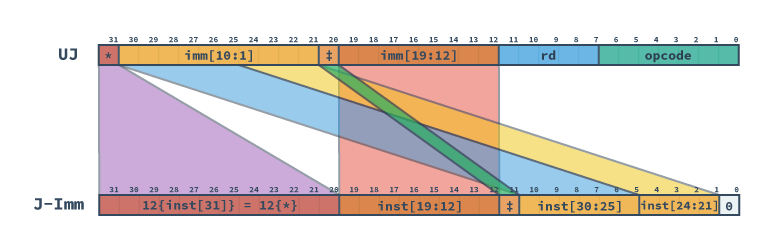
\includegraphics[width=1\linewidth]{figs/RV_J_Imm.png}
            \caption{Formação do Imediato de tipo J.}\label{fig:riscv_j_imm}
        \end{figure}


        % \begin{figure}[H]
        % \centering
        %     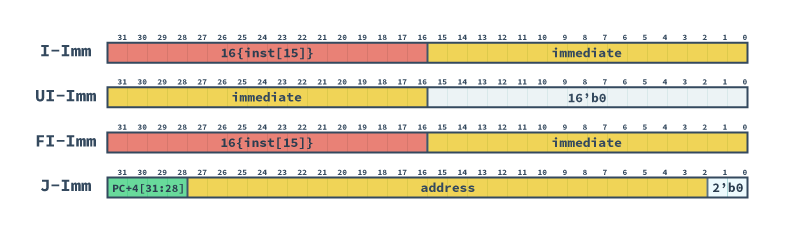
\includegraphics[width=1\linewidth]{figs/MIPS_Immediates.png}
        %     \caption{Formatos de Imediato da \textit{ISA MIPS32}.}\label{fig:mips_immediates}
        % \end{figure}

\chapter{Implementação}

\label{CapImpl}

% Resumo opcional. Comentar se não usar.
%\resumodocapitulo{Resumo opcional}

\chapter{Resultados}\label{CapResult}

% Resumo opcional. Comentar se não usar.
%\resumodocapitulo{Resumo opcional}


\chapter{Conclusões}

\label{CapConclusoes}

Concluir


\section{Perspectivas Futuras}

Perspectivas futuras



% Bibliografia
\renewcommand{\bibname}{REFERÊNCIAS BIBLIOGRÁFICAS}
\addcontentsline{toc}{chapter}{REFERÊNCIAS BIBLIOGRÁFICAS}

\bibliographystyle{abnt-num}
\bibliography{bibliography}


% Anexos
\anexos{}
\makeatletter
% não retirar estes comandos
\renewcommand{\@makechapterhead}[1]{%
  {\parindent \z@ \raggedleft \setfontarial\bfseries
\LARGE \thechapter. \space\space
\uppercase{#1}\par
\vskip 40\p@
}
}
\makeatother


% Anexo I: Descrição do CD

\chapter{Descrição do conteúdo do CD}

\label{AnCD} 

Descrever CD.


\refstepcounter{noAnexo}


% Anexo II: Programas Utilizados

\chapter{Programas utilizados}

Quais programas foram utilizados?


\refstepcounter{noAnexo}


% Acrescente mais anexos conforme julgar necessário.

\end{document}
